\documentclass[xcolor=dvipsnames,table]{beamer}

\usepackage{latexsym}
\usepackage[utf8]{inputenc}
\usepackage[brazil]{babel}
\usepackage{amssymb}
\usepackage{amsmath}
\usepackage{stmaryrd}
\usepackage{fancybox}
\usepackage{datetime}
\usepackage[T1]{fontenc}
\usepackage{graphicx}
\usepackage{graphics}
\usepackage{url}
\usepackage{algorithmic}
\usepackage{algorithm}
\usepackage{acronym}
\usepackage{array}

\usepackage{listings}
\usepackage{color}

\definecolor{mygreen}{rgb}{0,0.6,0}
\definecolor{mygray}{rgb}{0.5,0.5,0.5}
\definecolor{mymauve}{rgb}{0.58,0,0.82}

\lstdefinelanguage{JavaScript}{
  keywords={typeof, new, true, false, catch, function, return, null, catch, switch, var, if, in, while, do, else, case, break},
  keywordstyle=\color{blue}\bfseries,
  ndkeywords={class, export, boolean, throw, implements, import, this},
  ndkeywordstyle=\color{darkgray}\bfseries,
  identifierstyle=\color{black},
  sensitive=false,
  comment=[l]{//},
  morecomment=[s]{/*}{*/},
  commentstyle=\color{purple}\ttfamily,
  stringstyle=\color{red}\ttfamily,
  morestring=[b]',
  morestring=[b]",
}

\lstset{ %
  backgroundcolor=\color{white},   % choose the background color; you must add \usepackage{color} or \usepackage{xcolor}
  basicstyle=\small,        % the size of the fonts that are used for the code
  breakatwhitespace=false,         % sets if automatic breaks should only happen at whitespace
  breaklines=true,                 % sets automatic line breaking
  captionpos=b,                    % sets the caption-position to bottom
  commentstyle=\color{mygreen},    % comment style
  deletekeywords={...},            % if you want to delete keywords from the given language
  escapeinside={\%*}{*)},          % if you want to add LaTeX within your code
  extendedchars=true,              % lets you use non-ASCII characters; for 8-bits encodings only, does not work with UTF-8
  frame=single,	                   % adds a frame around the code
  keepspaces=true,                 % keeps spaces in text, useful for keeping indentation of code (possibly needs columns=flexible)
  keywordstyle=\color{blue},       % keyword style
  language=HTML,                 % the language of the code
  otherkeywords={*,...},           % if you want to add more keywords to the set
  numbers=left,                    % where to put the line-numbers; possible values are (none, left, right)
  numbersep=5pt,                   % how far the line-numbers are from the code
  numberstyle=\tiny\color{mygray}, % the style that is used for the line-numbers
  rulecolor=\color{black},         % if not set, the frame-color may be changed on line-breaks within not-black text (e.g. comments (green here))
  showspaces=false,                % show spaces everywhere adding particular underscores; it overrides 'showstringspaces'
  showstringspaces=false,          % underline spaces within strings only
  showtabs=false,                  % show tabs within strings adding particular underscores
  stepnumber=1,                    % the step between two line-numbers. If it's 1, each line will be numbered
  stringstyle=\color{mymauve},     % string literal style
  tabsize=2,	                   % sets default tabsize to 2 spaces
  title=\lstname,                   % show the filename of files included with \lstinputlisting; also try caption instead of title
  moredelim=**[is][\color{purple}]{@}{@},
}

\newtheorem{definicao}{Definio}
\newcommand{\tab}{\hspace*{2em}}

\mode<presentation>
{
  \definecolor{colortexto}{RGB}{0,0,0}
 
  \setbeamertemplate{background canvas}[vertical shading][ bottom=white!10,top=white!10]
  \setbeamercolor{normal text}{fg=colortexto} 

  \usetheme{Warsaw}
}

\title{JavaScript (Parte 3)} 

\author{
  Esdras Lins Bispo Jr. \\ \url{bispojr@ufg.br}
  } 
 \institute{
  Física para Ciência da Computação \\Bacharelado em Ciência da Computação}
\date{\textbf{09 de setembro de 2019} }

\logo{
\includegraphics[width=1cm]{images/ufgJataiLogo.png}}

\begin{document}

	\begin{frame}
		\titlepage
	\end{frame}

	\AtBeginSection{
		\begin{frame}{Sumário}%[allowframebreaks]{Sumário}
    		\tableofcontents[currentsection]
    		%\tableofcontents[currentsection, hideothersubsections]
		\end{frame}
	}

	\begin{frame}{Plano de Aula}
		\tableofcontents
		%\tableofcontents[hideallsubsections]
	\end{frame}
	
	\section{Revisão}
		
\begin{frame}[fragile]{Funções e Métodos}
	\begin{block}{Atribuindo uma função como propriedade de um objeto...}
		\begin{lstlisting}[language=JavaScript]
nomeDoObjeto.nomeDaPropriedade = nomeDaFuncao;
\end{lstlisting}	
	\end{block} 
	\begin{block}{Exemplo}
		\begin{lstlisting}[language=JavaScript]
obj.multiplicar = multiplicar;
\end{lstlisting}	
	\end{block}
\end{frame}

\subsection{Herança, Construtores e Protótipos}
\begin{frame}{Herança}
	\begin{center}
		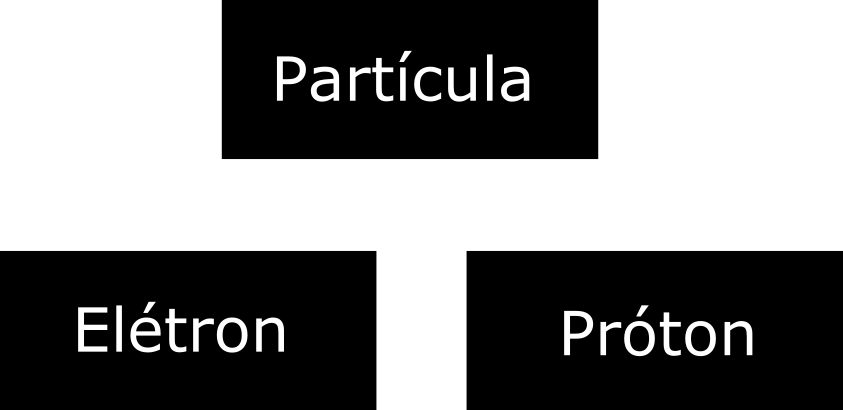
\includegraphics[scale=0.3]{images/heranca01.png}
	\end{center}
\end{frame}

\begin{frame}{Herança}
	\begin{center}
		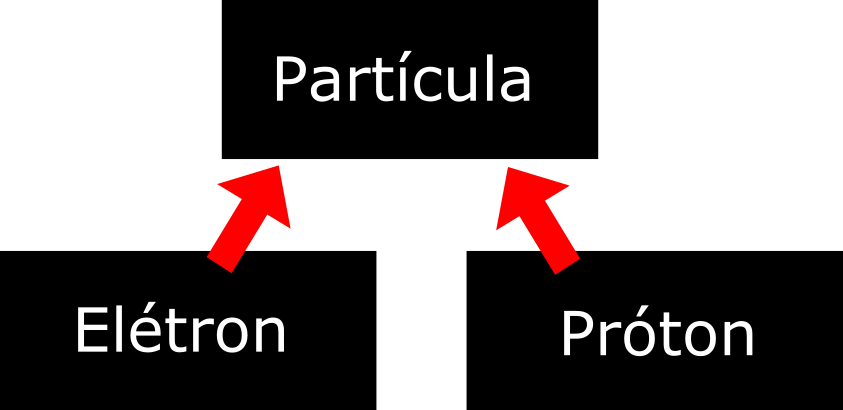
\includegraphics[scale=0.3]{images/heranca02.png}
	\end{center}
\end{frame}

\begin{frame}{Herança}
	\begin{center}
		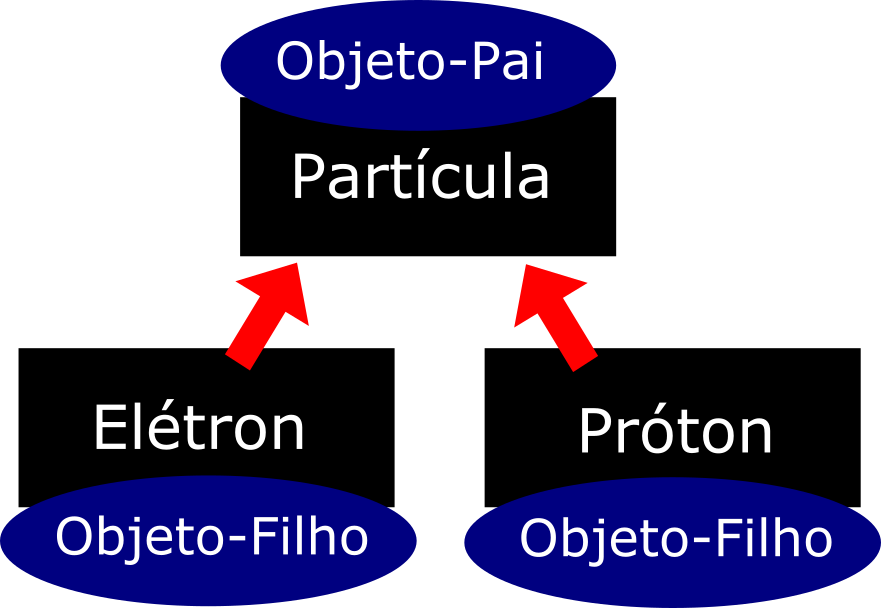
\includegraphics[scale=0.3]{images/heranca03.png}
	\end{center}
\end{frame}

\begin{frame}[fragile]{Construtor}
	\begin{block}{Objeto a partir de uma função}
		É possível construir um objeto a partir de uma ``função-modelo''.
		\begin{lstlisting}[language=JavaScript]
function Particula(pnome){
	this.nome = pnome;
	this.mover = function(){
		console.log(this.nome + " em movimento!");
	};
}
\end{lstlisting}	
	\end{block}
\end{frame}

\begin{frame}[fragile]{Construtor}
	\begin{block}{Objeto a partir de uma função}
		\begin{lstlisting}[language=JavaScript]
particula1 = new Particula("eletron");
console.log(particula1.nome); //exibe "eletron"
particula1.mover();	
			//exibe "eletron em movimento"
\end{lstlisting}	
	\end{block}
	\begin{block}{Construtor...}
		Se uma função é utilizada intencionalmente para criar novos objetos, a chamamos de {\bf construtor}.
	\end{block}
\end{frame}

\begin{frame}[fragile]{Protótipo}
	\begin{block}{Adicionando propriedades...}
		Após declarado, é possível adicionar propriedades a um construtor.
		\begin{lstlisting}[language=JavaScript]
Particula.prototype.massa = 1;
Particula.prototype.parar = 
		function(){console.log("Eu parei.");};
\end{lstlisting}	
	\end{block} 
	\begin{block}{Para novos objetos...}
		\begin{lstlisting}[language=JavaScript]
particula2 = new Particula("proton");
console.log(particula2.massa); //exibe 1
\end{lstlisting}	
	\end{block}
\end{frame}

\begin{frame}[fragile]{Protótipo}
	\begin{block}{Entretanto...}
		\begin{lstlisting}[language=JavaScript]
particula3 = new Particula("neutron");
particula3.massa = 2;	//propriedade com valor 2
console.log(Particula.prototype.massa);	//exibe 1
\end{lstlisting}	
	\end{block} 
	\begin{alertblock}{Necessário ter em mente...}
		A propriedade {\tt prototype} modifica o objeto-pai.	
	\end{alertblock}
\end{frame}

\begin{frame}[fragile]{Protótipo}
	\begin{block}{Algo interessante...}
		É possível adicionar propriedades apenas para o objeto-filho.
		\begin{lstlisting}[language=JavaScript]
particula4 = new Particula("neutrino");
particula4.spin = 0; //exibe 0
\end{lstlisting}	
	\end{block}
\end{frame}

\begin{frame}[fragile]{Exemplo...}
	\begin{block}{Objeto Bola}
		\begin{lstlisting}[language=JavaScript]
function Bola (raio, cor) {
	this.raio = raio;
	this.cor = cor;
	this.x = 0;
	this.y = 0;
	this.vx = 0;
	this.vy = 0;
}
\end{lstlisting}	
	\end{block}
\end{frame}

\begin{frame}[fragile]{Exemplo...}
	\begin{block}{Objeto Bola}
		\begin{lstlisting}[language=JavaScript]
Bola.prototype.desenhar = function (contexto) {
	contexto.fillStyle = this.cor;
	contexto.beginPath();
	contexto.arc(this.x, this.y, 
							this.raio, 0, 2*Math.PI, true);
	contexto.closePath();
	contexto.fill();
};
\end{lstlisting}	
	\end{block}
\end{frame}

\begin{frame}[fragile]{Exemplo...} 
	\begin{block}{HTML Canvas {\tt arc}}
		A propriedade {\tt arc()} cria um arco \\(utilizado para criar círculos ou parte de círculos). 
	\end{block}
	\begin{block}{Sintaxe}
		{\tt arc(x, y, raio, angIni, angFin, antiHor);}
	\end{block}
	\begin{block}{Argumentos}
		\begin{itemize}
			\item {\tt x} e {\tt y}: coordenadas do arco;
			\item {\tt raio}: raio do arco; 
			\item {\tt angIni} e {\tt angFin}: ângulos inicial e final do arco \\(em radianos);
			\item {\tt antiHor}: valor booleano para o sentido anti-horário.
		\end{itemize}
	\end{block}
\end{frame}

\begin{frame}{Exemplo...}
	\begin{center}
		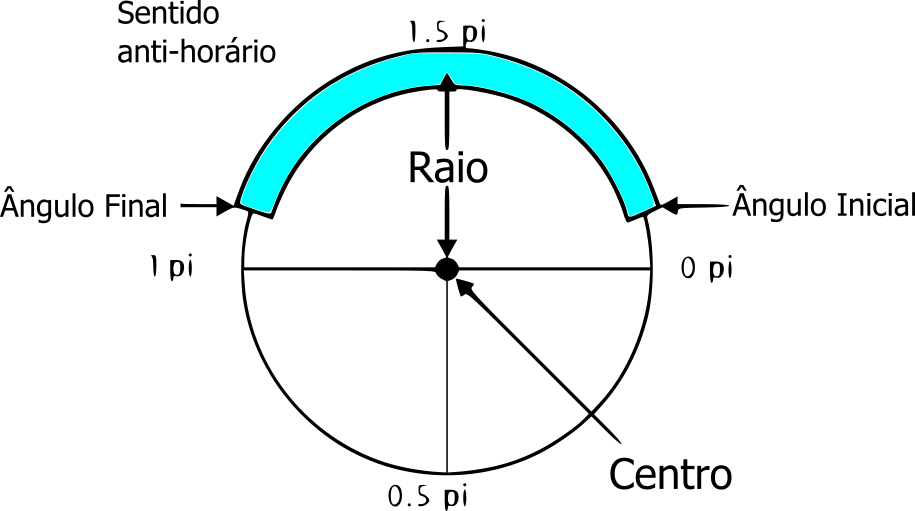
\includegraphics[scale=0.4]{images/arc.png}
	\end{center}
\end{frame}

\begin{frame}[fragile]{Exemplo...}
	\begin{block}{Objeto Bola}
		\begin{lstlisting}[language=JavaScript]
var canvas = document.getElementById('canvas');
var contexto = canvas.getContext('2d');
var bola = new Bola(50,'#0000ff');
bola.x = 100;
bola.y = 100;
bola.desenhar(contexto);
\end{lstlisting}	
	\end{block}
\end{frame}

\section{Conceitos Básicos em JavaScript}
\begin{frame}[fragile]{Conceitos Básicos em JavaScript}
	\begin{block}{Variáveis}
		Uma {\bf variável} funciona como uma caixa que armazena valores de dados.
	\end{block} \pause
	\begin{block}{Exemplo}
		\begin{lstlisting}[language=JavaScript]
var x;
x = 2;
var y = 3;
z = 2*x + y;	//z - variavel global
x = x + 1;
\end{lstlisting}	
	\end{block}
\end{frame}

\begin{frame}[fragile]{Conceitos Básicos em JavaScript}
	\begin{block}{Tipos de Dados}
		\begin{itemize}
			\item Variáveis em JavaScript têm tipos de dados dinâmicos; \pause
			\item i.e., podem armazenar tipos de dados diferentes em momentos diferentes.
		\end{itemize}
	\end{block} \pause
	\begin{block}{Descrição}
		\begin{itemize}
			\item {\tt Number}: número de ponto flutuante com dupla precisão de 64 bits. \pause
			\item {\tt String}: uma sequência de caracteres de 16 bits. \pause
			\item {\tt Boolean}: tem dois valores possíveis: {\tt true} e {\tt false}, ou 1 e 0. \pause
			\item {\tt Undefined}: é retornado para uma propriedade de objeto não-existente ou uma variável sem um valor. \pause
			\item {\tt Null}: tem apenas um valor $\rightarrow$ {\tt null}
		\end{itemize}	
	\end{block}
\end{frame}


\begin{frame}[fragile]{Conceitos Básicos em JavaScript}
	\begin{block}{Descrição}
		\begin{itemize}
			\item {\tt Object}: armazena uma coleção de propriedades e métodos. \pause
			\item {\tt Array}: um objeto consistindo de uma lista de dados de algum tipo. \pause 
			\item {\tt Function}: um objeto passível de ser chamado, que executa um bloco de código. 
		\end{itemize}	
	\end{block}
\end{frame}

\begin{frame}[fragile]{Conceitos Básicos em JavaScript}
\begin{block}{Números}
	\begin{itemize}
		\item Existe um único tipo de dado numérico em JavaScript: {\tt Number}; \pause
		\item Não há diferença entre números inteiros e pontos-flutuantes, por exemplo; \pause 
		\item O maior valor que {\tt Number} pode armazenar é $1,8 \times 10^{308}$; \pause
		\item O número de átomos do universo visível é estimado em $10^{80}$; \pause
		\item Permite armazenar números bem pequenos como $5 \times 10^{-324}$.
	\end{itemize}	
\end{block} \pause
\begin{block}{Valores especiais em {\tt Number}}
	\begin{itemize}
		\item {\tt NaN} (Not a Number): e.g. raiz de -1, ou 0/0; \pause
		\item {\tt Infinity} e {\tt -Infinity}: divisão de um valor não-zero por zero (e.g. 5/0 ou (-3)/0).
	\end{itemize}
\end{block}
\end{frame}

\begin{frame}[fragile]{Conceitos Básicos em JavaScript}
\begin{block}{Strings}
Uma {\bf string} é uma sequência de caracteres. Normalmente, vem delimitada por aspas (simples ou dupla).
\end{block} \pause
\begin{block}{Exemplo}
\begin{lstlisting}[language=JavaScript]
var str = "Olah jovens";
console.log(str);
\end{lstlisting}	
\end{block}
\end{frame}

\begin{frame}[fragile]{Conceitos Básicos em JavaScript}
\begin{block}{Booleanos}
Um {\bf booleano} pode ter apenas dois valores: {\tt true} ou {\tt false}.
\end{block} \pause
\begin{block}{Exemplo}
\begin{lstlisting}[language=JavaScript]
var bln = false;	// valor booleano false
bln = "true";		// string "true"... cuidado!
\end{lstlisting}	
\end{block}
\end{frame}

\begin{frame}[fragile]{Conceitos Básicos em JavaScript}
\begin{block}{\tt Undefined}
\begin{itemize}
\item O tipo de dados {\tt Undefined} tem um único valor: {\tt undefined}. \pause
\item Casos que uma variável assume {\tt undefined}: \pause
\begin{itemize}
\item Propriedade inexistente; \pause
\item Variável declarada, mas não inicializada; \pause
\item Função sem {\tt return}; \pause
\item Argumento não fornecido de uma função.
\end{itemize}
\end{itemize}
\end{block} 
\end{frame}

\begin{frame}[fragile]{Conceitos Básicos em JavaScript}
\begin{block}{\tt Null}
\begin{itemize}
\item O tipo de dados {\tt Null} tem um único valor: {\tt null}. \pause
\item Diferença crucial entre {\tt null} e {\tt undefined}: {\tt null} é associado a variável de forma proposital.
\end{itemize}	
\end{block} \pause
\begin{block}{Exemplo}
\begin{lstlisting}[language=JavaScript]
var noVal = null;
console.log(typeof noVal);	// retorna "Object"
\end{lstlisting}	
\end{block}
\end{frame}

\begin{frame}[fragile]{Conceitos Básicos em JavaScript}
\begin{block}{Vetores}
Um vetor é uma coleção de objetos.	
\end{block} \pause
\begin{block}{Exemplo 1}
\begin{lstlisting}[language=JavaScript]
var arr = new Array();
arr = [2, 4, 6];
console.log(arr[1]); // imprime 4
arr[3] = 8;	// 8 - quarto elemento do vetor
\end{lstlisting}	
\end{block}
\end{frame}

\begin{frame}[fragile]{Conceitos Básicos em JavaScript}
\begin{block}{Exemplo 2}
\begin{lstlisting}[language=JavaScript]
var xArr = new Array();
var yArr = new Array();
xArr = [1,2];
yArr = [3,4];
var zArr = new Array(xArr,yArr);
console.log( zArr[0][1] ); // retorna 2
console.log( zArr[1][0] ); // retorna 3
\end{lstlisting}	
\end{block}
\end{frame}

\begin{frame}[fragile]{Conceitos Básicos em JavaScript}
\begin{block}{Operadores (Exemplo 1)}
\begin{lstlisting}[language=JavaScript]
var x = 5;
var y = 3;
x%y; // retorna 2
var z;
z = x++; // atribui o valor de x a z, e depois incrementa x
console.log(z); // retorna 5
z = ++x; // incrementa o valor de x, e depois atribui-o a z
console.log(z); //retorna 7
\end{lstlisting}	
\end{block}
\end{frame}

\begin{frame}[fragile]{Conceitos Básicos em JavaScript}
\begin{block}{Operadores (Exemplo 2)}
\begin{lstlisting}[language=JavaScript]
var a = 1;
a = a + 1;
console.log(a); // retorna 2
a += 1; // forma reduzida de a = a + 1
console.log(a); // retorna 3
a = 4*a;
console.log(a); // retorna 12
a *= 4; // forma reduzida de a = a*4
console.log(a); // retorna 48
\end{lstlisting}	
\end{block}
\end{frame}

\begin{frame}[fragile]{Conceitos Básicos em JavaScript}
\begin{block}{Alguns métodos matemáticos...}
\begin{itemize}
\item {\tt Math.abs(a)}: valor absoluto de {\tt a}; \pause
\item {\tt Math.pow(a,b)}: {\tt a} elevado à potência de {\tt b}; \pause
\item {\tt Math.sqrt(a)}: raiz quadrada de {\tt a}; \pause
\item {\tt Math.ceil(a)}: o menor inteiro que é maior que {\tt a}; \pause
\item {\tt Math.floor(a)}: o maior inteiro que é menor que {\tt a}; \pause
\item {\tt Math.round(a)}: o inteiro mais próximo de {\tt a}; \pause 
\item {\tt Math.max(a,b,c,...)}: o maior entre {\tt a, b, c, ...}; \pause
\item {\tt Math.min(a,b,c,...)}: o menor entre {\tt a, b, c, ...}; \pause
\item {\tt Math.random()}: um número pseudo-aleatório {\tt n}, em que $0 \leq n < 1$.
\end{itemize}
\end{block}
\end{frame}

\begin{frame}[fragile]{Conceitos Básicos em JavaScript}
\begin{block}{Exemplo com {\tt Math.random()}}
\begin{lstlisting}[language=JavaScript]
vx = Math.random()*5;	// 0 <= n < 5
vy = (Math.random()-0.5)*4;	// -2 <= n < 2
\end{lstlisting}	
\end{block}
\end{frame}

\begin{frame}[fragile]{Conceitos Básicos em JavaScript}
\begin{block}{Outros exemplos...}
\begin{lstlisting}[language=JavaScript]
if (a == 0){
	// faca algo se a=0
} else if (a < 0 ) {
	// faca algo caso a seja negativo
} else if (a > 0) {
	// faca algo caso a seja positivo
} else {
	// faca algo caso o valor de a seja um NaN
}
\end{lstlisting}	
\end{block}
\end{frame}

\begin{frame}[fragile]{Conceitos Básicos em JavaScript}
\begin{block}{Outros exemplos...}
\begin{lstlisting}[language=JavaScript]
var sum = 0;
for (var i = 1; i <= 100; i++) {
	sum += i;
}
console.log(sum);
\end{lstlisting}	
\end{block}
\end{frame}

\begin{frame}[fragile]{Conceitos Básicos em JavaScript}
\begin{block}{Outros exemplos...}
\begin{lstlisting}[language=JavaScript]
var sum = 0;
var i = 1;
while (i <= 100) {
	sum += i;
	i++;
}
console.log(sum);
\end{lstlisting}	
\end{block}
\end{frame}
	
	\begin{frame}
		\titlepage
	\end{frame}
	
\end{document}